\section{Estrutura}

\subsection{Maletas}

\subsubsection{Elementos estruturais}

\par O RGS necessita que todo o seu sistema seja portátil e suficiente para configurar e apoiar as missões de foguetes da CTR. Assim durante sua concepção estrutural o principal foco da equipe foi a mobilidade e a robustez para adequação às condições ambientais encontradas nos potenciais locais de lançamento e teste de foguetes. Por isso nossa estrutura deve ser equipada com todos os instrumentos necessários para o suporte eletrônico e de software responsáveis por rastrear e comandar o foguete durante o lançamento.


\par Como já dito o GCS precisava ser portátil assim uma case para comportar os equipamentos se faz necessária e esse se torna o primeiro elemento principal da área estrutural.

\par Depois tem-se a parte interna onde os componentes eletrônicos principais precisam ser inseridos, bem como um compartimento para o sistema de alimentação e um espaço de armazenamento para o sistema de abastecimento. Com isso percebe-se a necessidade do desenvolvimento de no mínimo três compartimentos isolados separados por divisórias na parte inferior da solução. Assim as divisórias internas são o segundo elemento estrutural de interesse. 

\par Além do que já foi dito se faz necessário o uso de uma placa para acomodar os equipamentos de acesso ao usuário, para tornar seu uso mais ergonômico, bem como uma placa na tampa superior com a mesma finalidade de separar os equipamentos de qual o usuário necessita ter acesso daqueles que são responsáveis pelo bom funcionamento do sistema. Se tornando assim terceiro elemento.

\par Para sua construção além das partes citadas que devem ser confeccionadas a partir do levantamento de materiais apresentados na seção \ref{sub:Especificações de materiais} se faz ainda necessário o uso de parafusos auto-roscantes com suas devidas arruelas, dobradiças, pegador e um material para isolamento que garanta a não interferência e vibração do sistema.

\par Algumas recomendações são para que durante o desenvolvimento do projeto, deixe-se devidamente marcado lugares e caminhos por onde os fios elétricos e eletrônicos deverão passar, além de serem etiquetados para manutenções futuras. Outra recomendação é que todo o seu processo de montagem se baseie em uma única ferramenta de montagem, exemplo uma chave de fenda universal para a GRS.

\subsubsection{Design conceitual}

\par Durante a concepção de um protótipo, os subsistemas que o compõem devem desenvolver os seus componentes em forma de desenho assistido por computador (CAD), para que possa ser realizada a integração das partes e obter um modelo tridimensional virtual que represente fielmente o projeto a ser executado. Além de ser possível incluir as dimensões e o formato geométrico, também pode-se configurar o tipo de material de cada peça. Com isso, é possível estimar parâmetros que serão usados de entrada para as simulações estruturais e  estimativa de preço.

\par Como o protótipo pode sofrer alterações ao longo do projeto, o desenho virtual se torna uma ferramenta conveniente para alterar e modificar o que for necessário para somente ser fabricado quando completamente finalizado os ajustes, evitando assim gastos desnecessários de tempo e de dinheiro.   

\par Levando-se em conta as soluções experimentais e comerciais encontradas, é proposto uma geometria retangular em forma de uma maleta. A maleta possui alças para facilitar seu transporte e dobradiças reguláveis que permitem sua abertura e fechamento. Na parte interior da maleta há um fundo falso que dá acesso a um pequeno compartimento de armazenamento, e garante acesso também aos equipamentos eletrônicos.

\begin{figure} [H]
\centering
  \subfigure[Fechada horizontal 01]{
    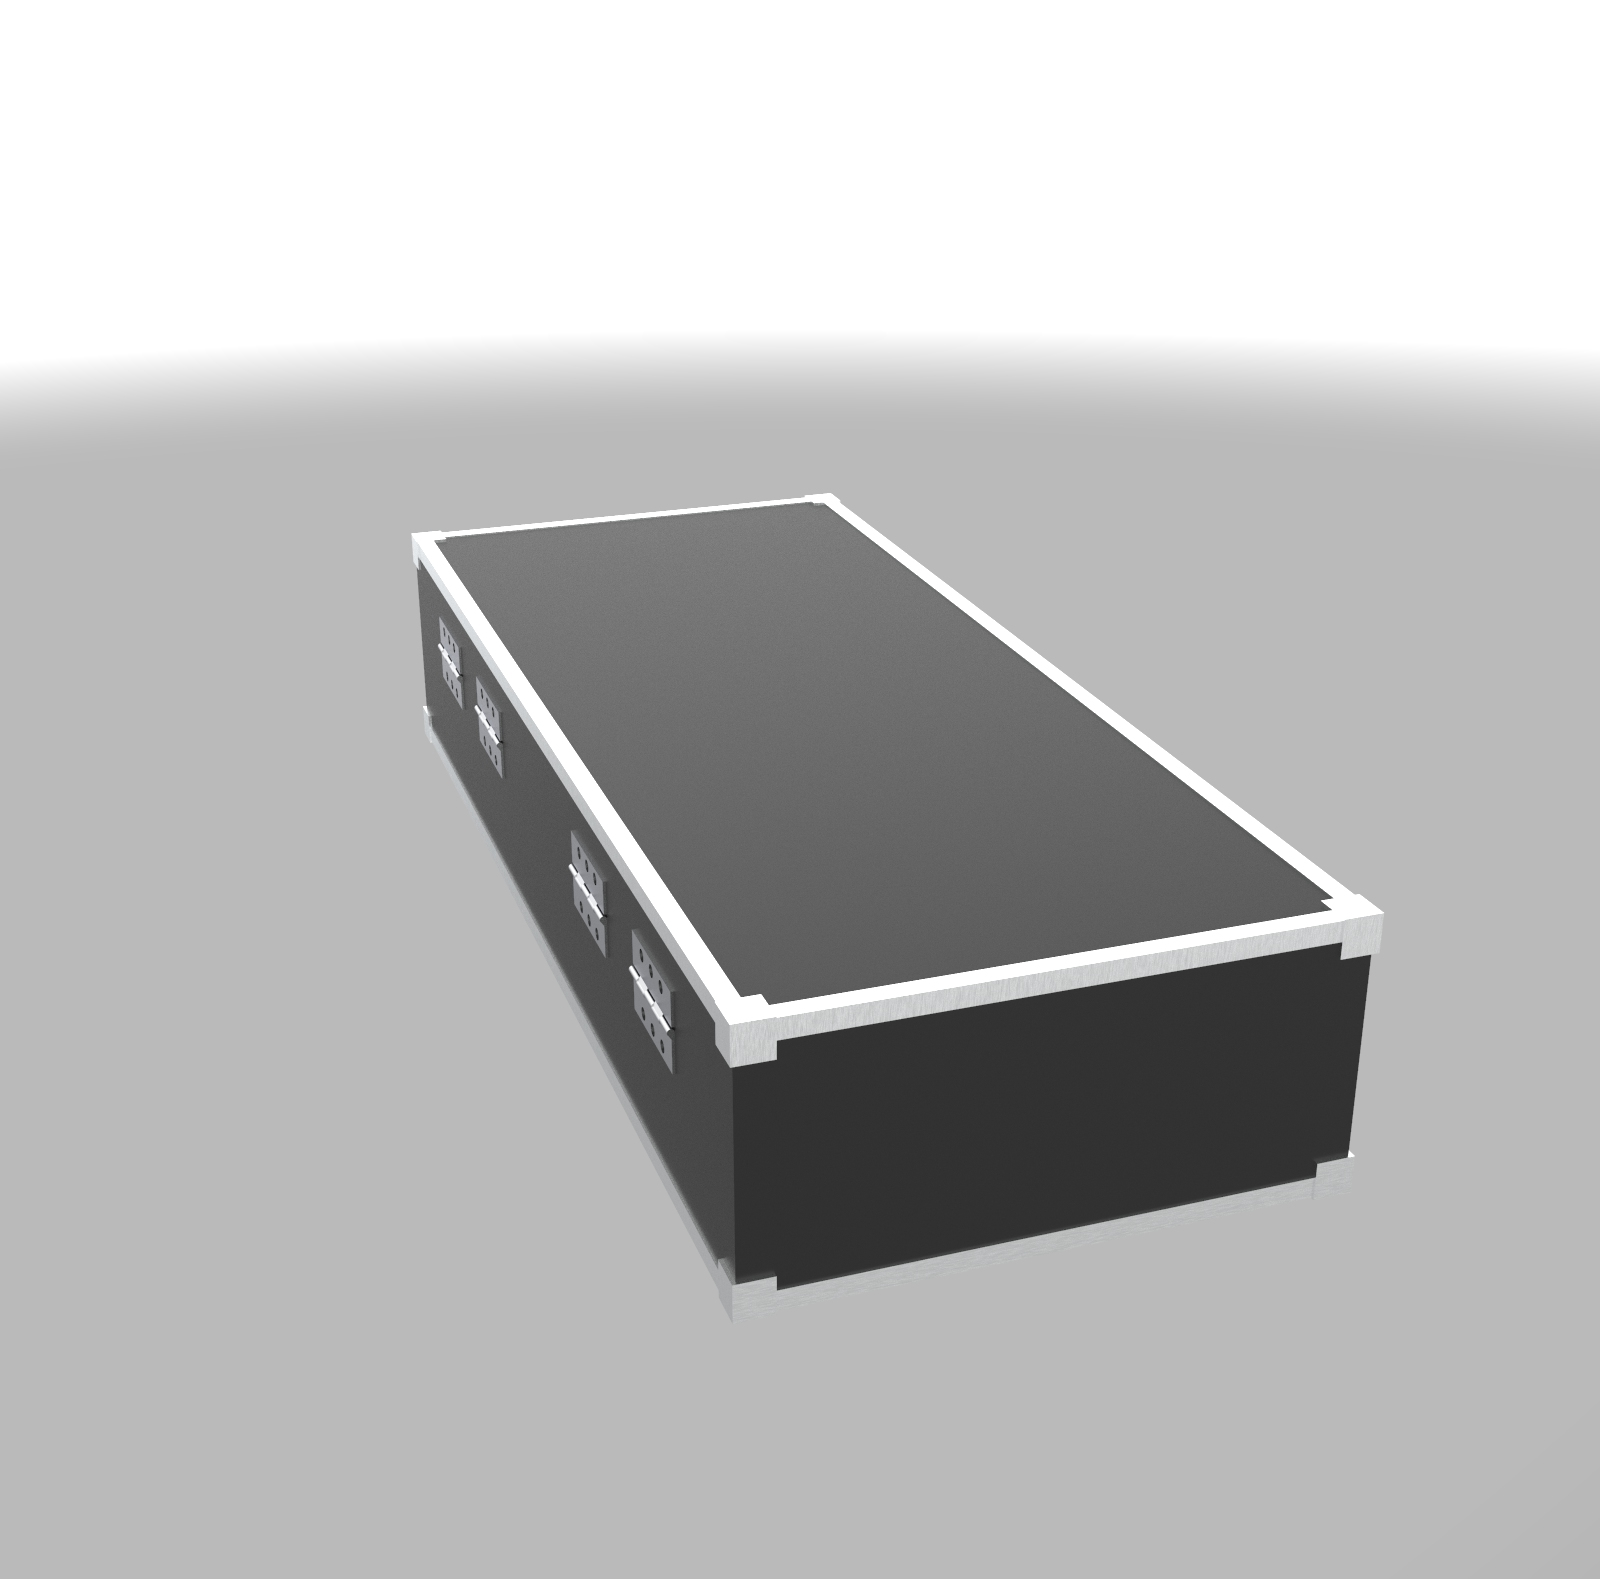
\includegraphics[width=7cm]{figuras/maletaiso_7}
  } 
  \subfigure[Fechada horizontal 02]{ 
    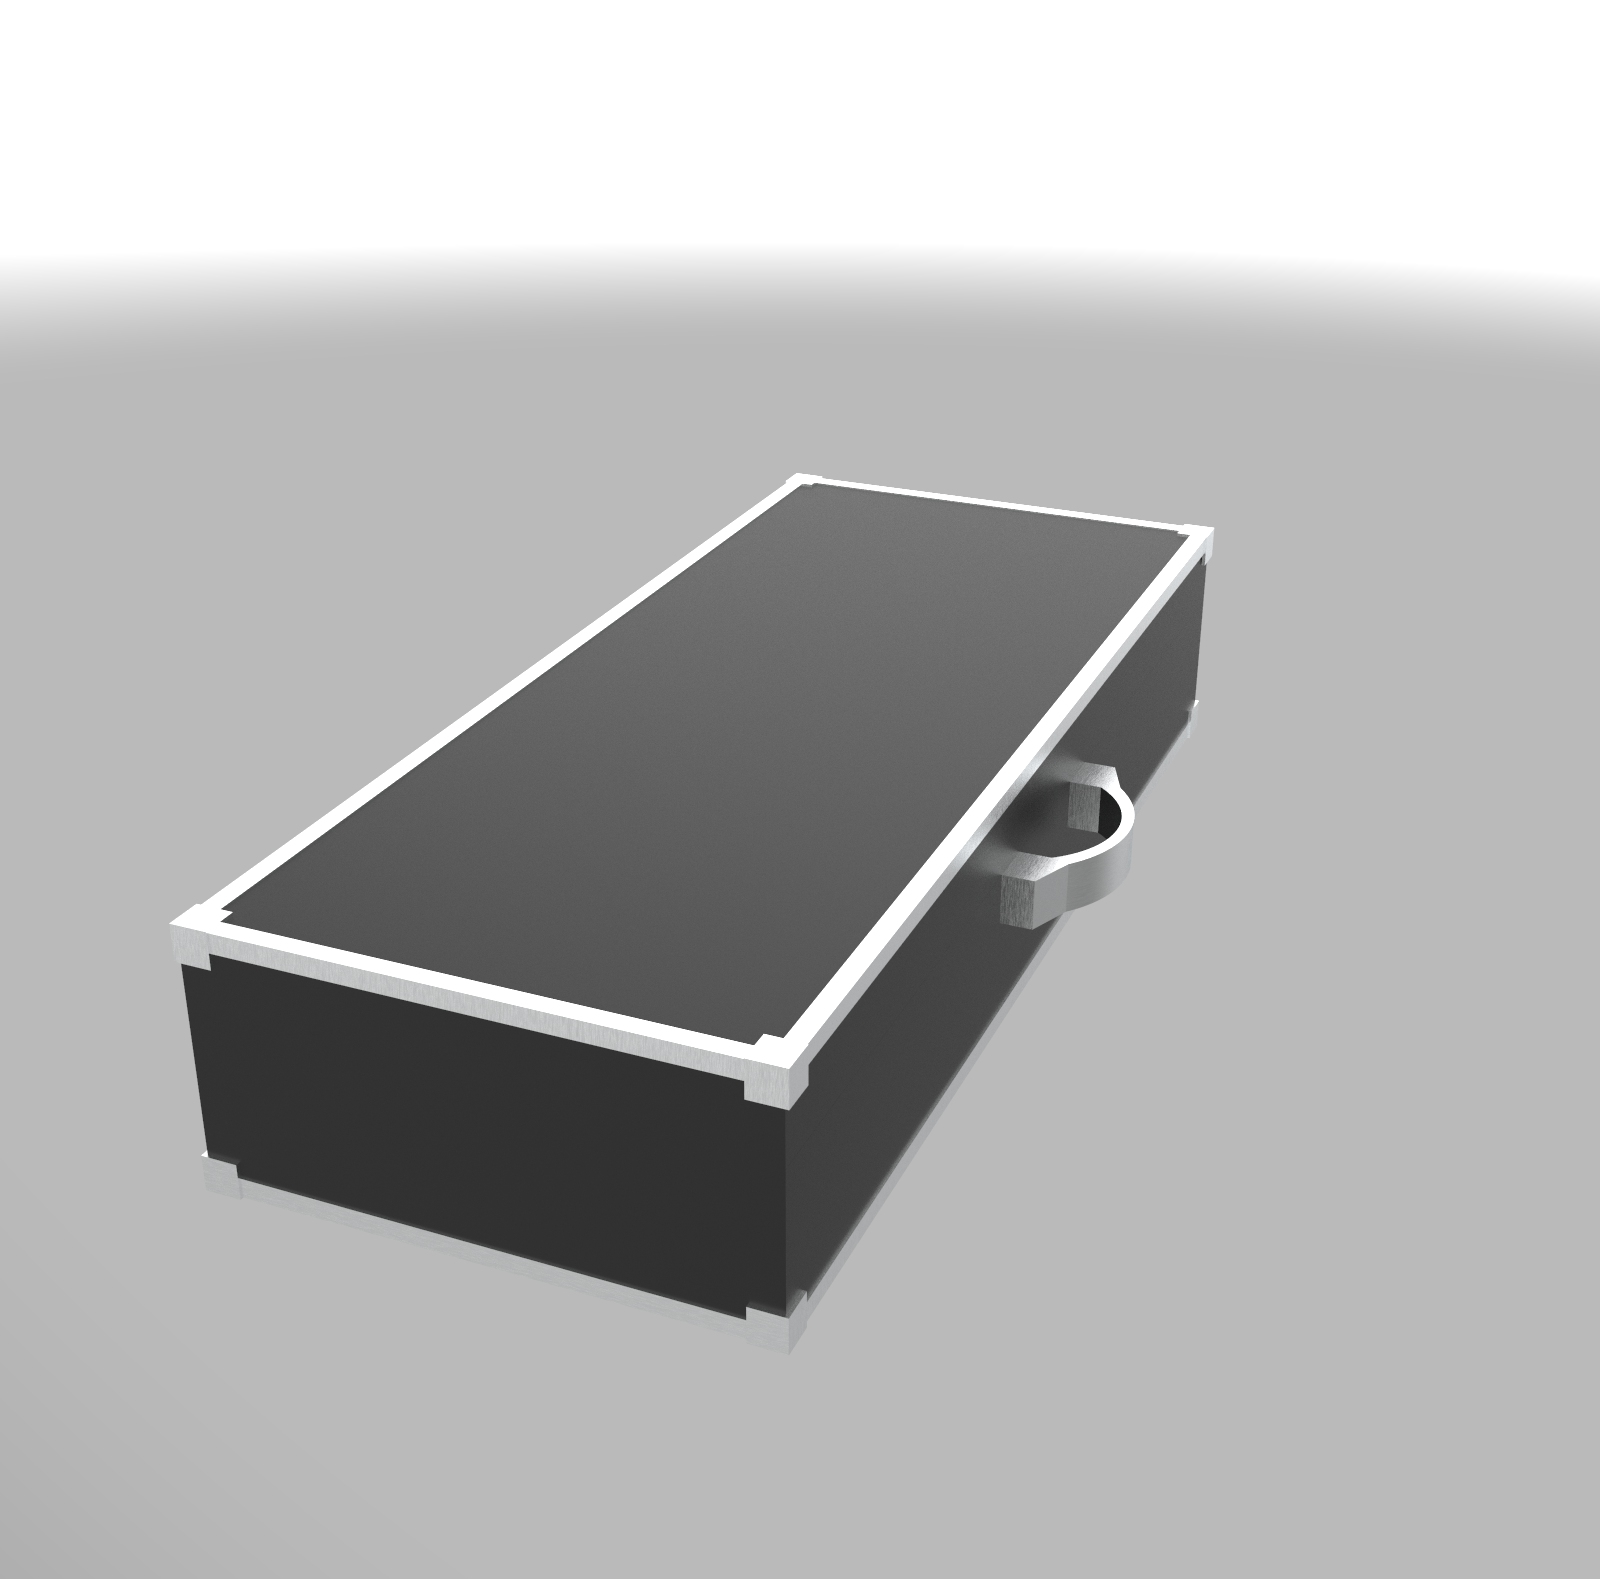
\includegraphics[width=7cm]{figuras/maletaiso_8}
  } 
  \\ 
  \subfigure[Fechada vertical]{
    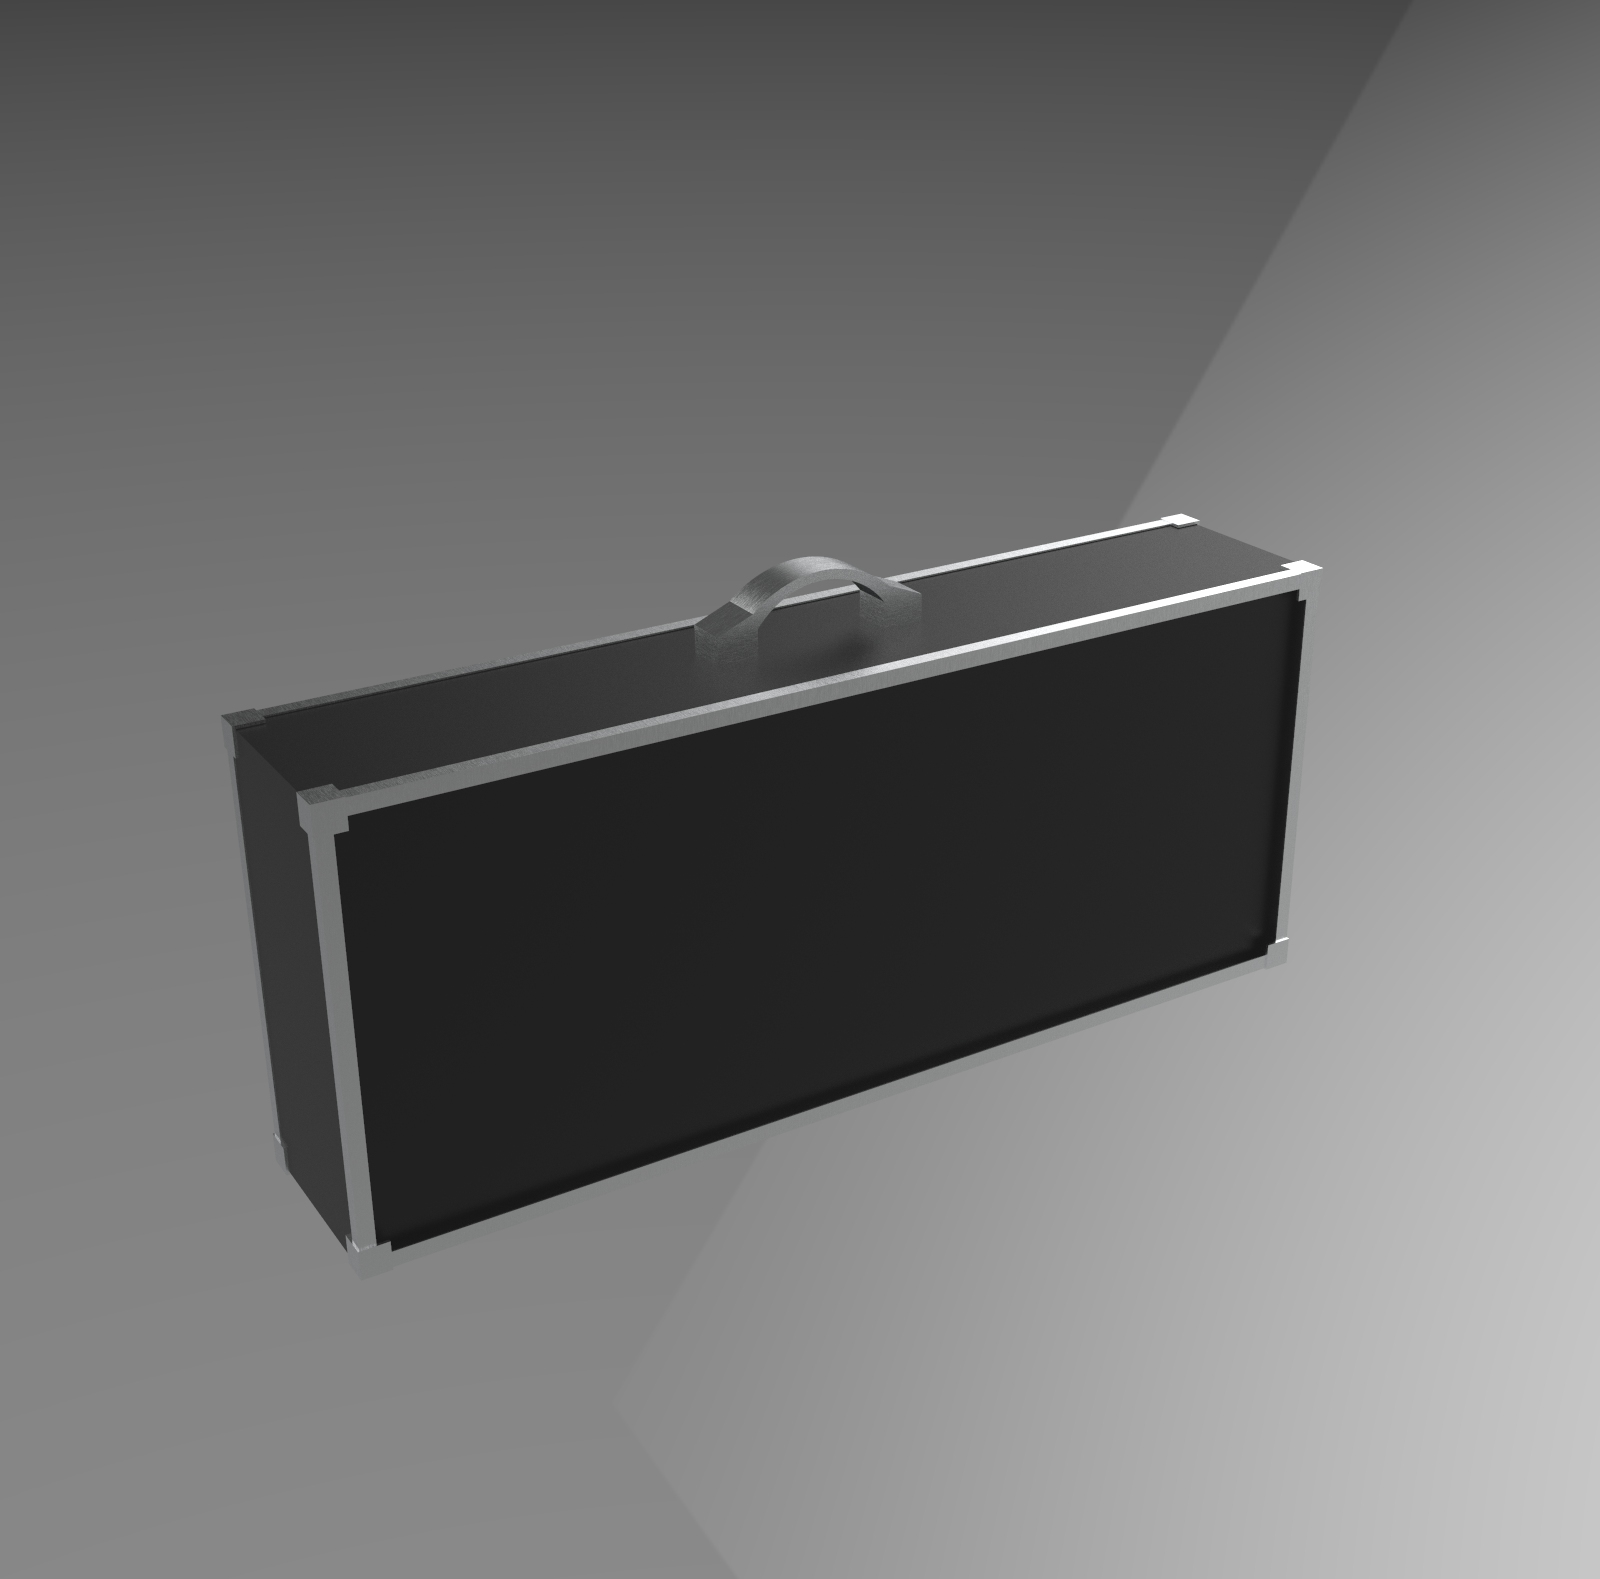
\includegraphics[width=7cm]{figuras/maletaiso_9}
  } 
  \subfigure[Visão lateral]{
    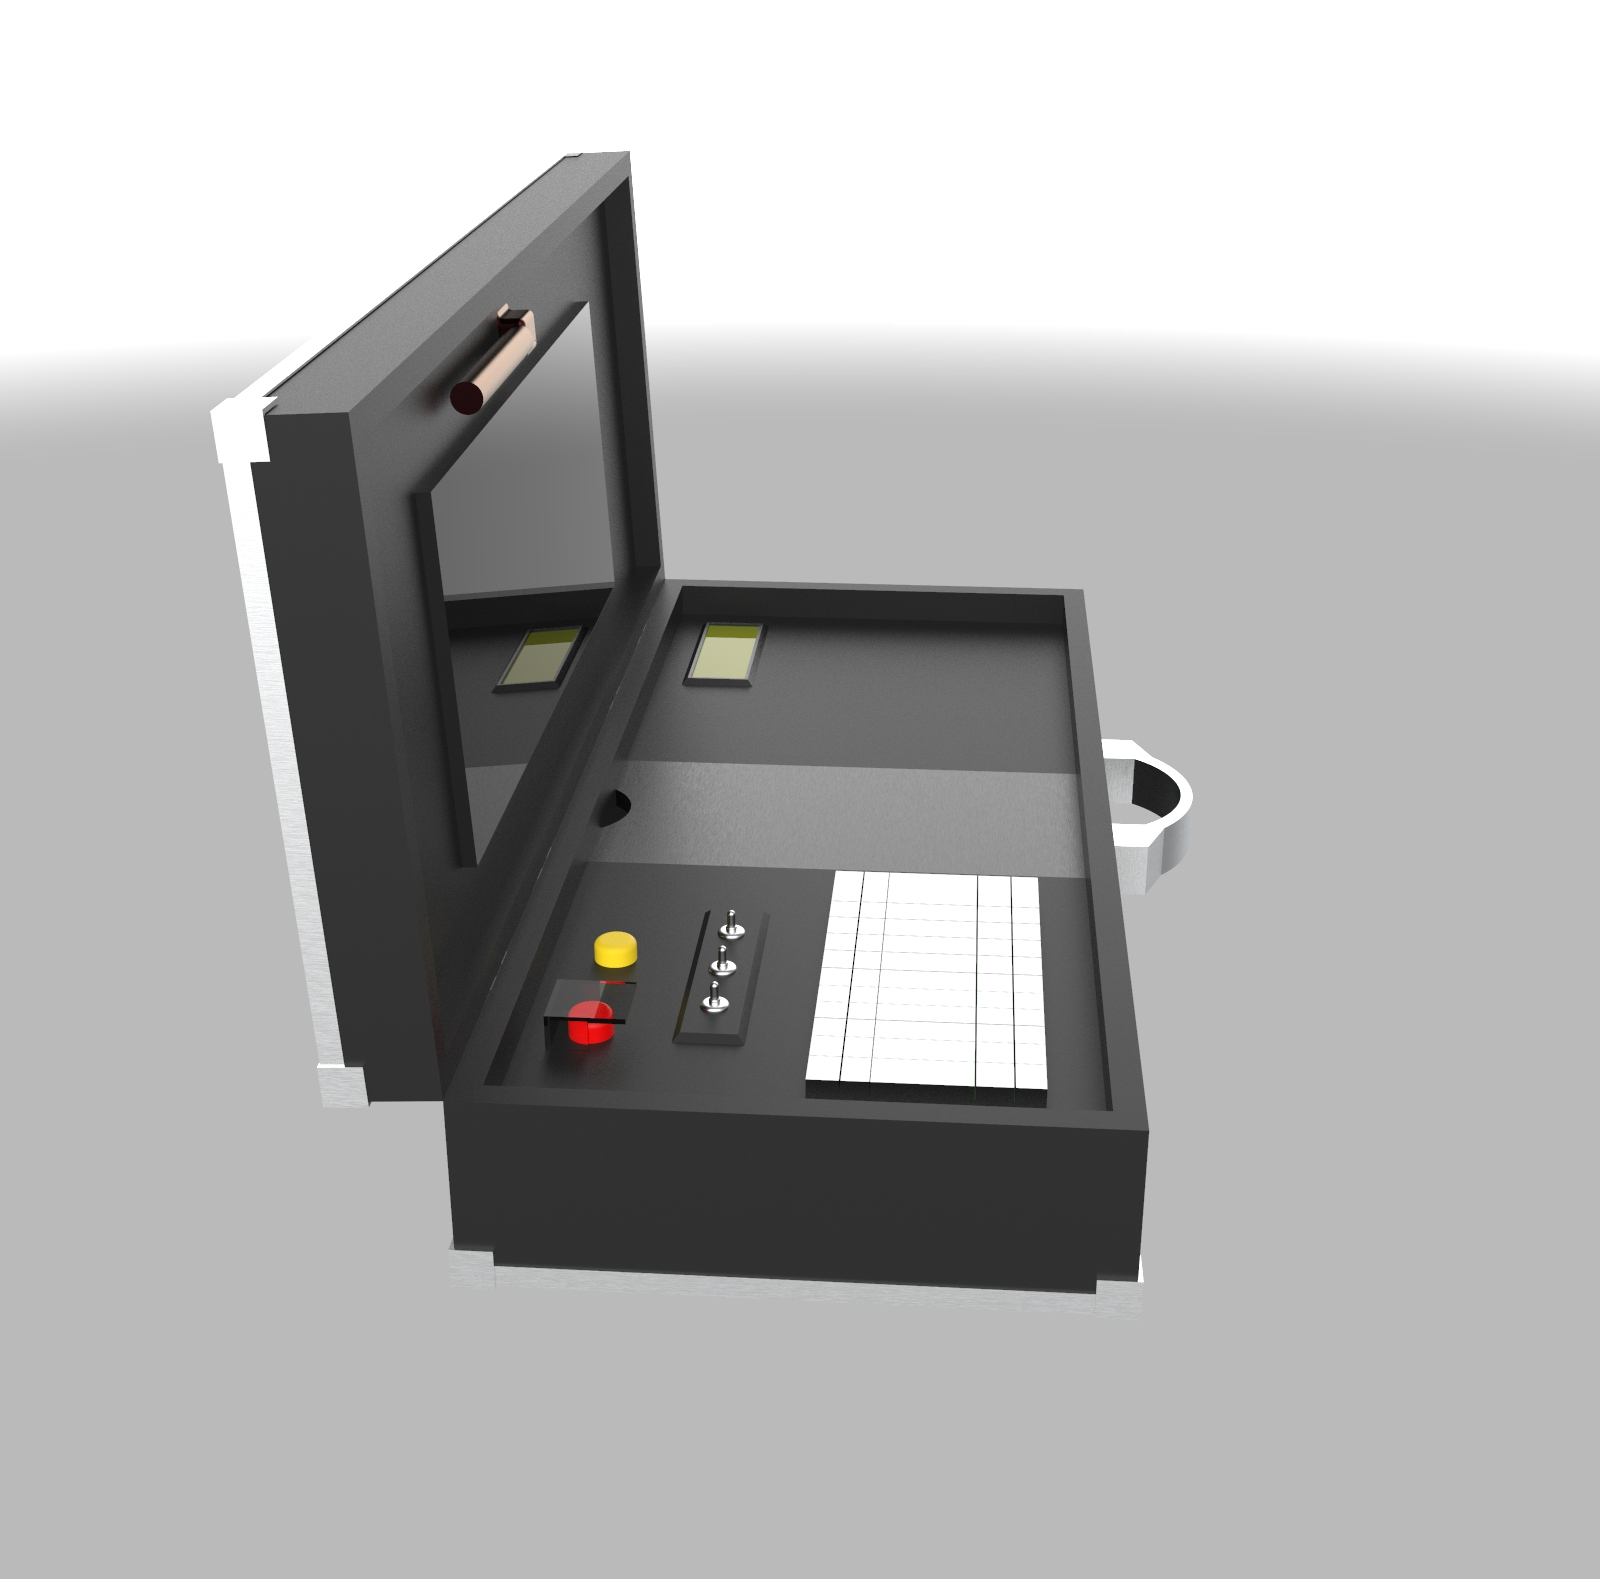
\includegraphics[width=7cm]{figuras/maletaiso_6}
  }
  \\ 
  \subfigure[Visão frontal]{
    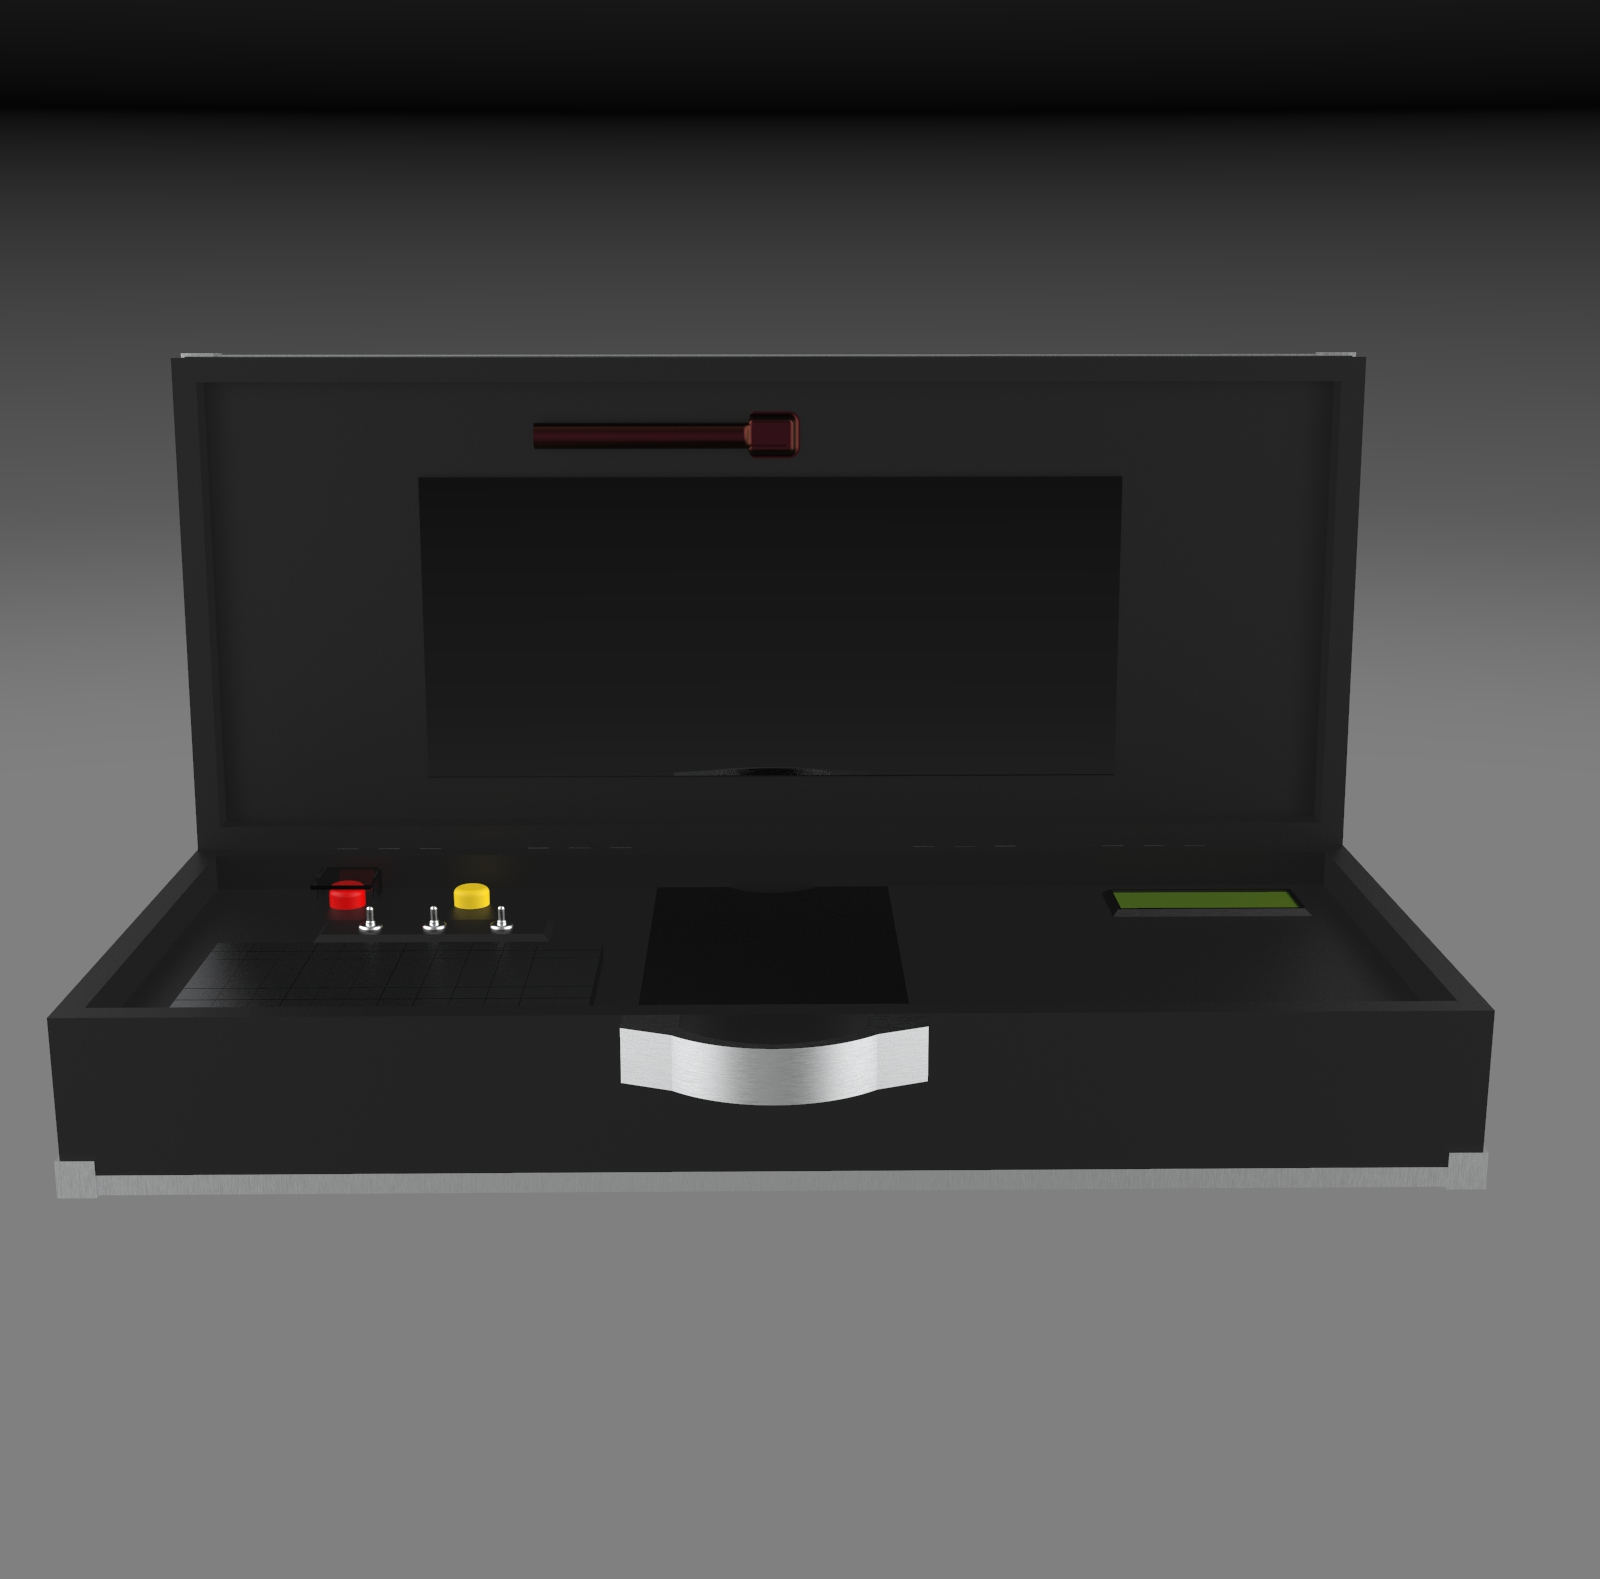
\includegraphics[width=7cm]{figuras/maletaiso_5}
  } 
  \caption{A maleta sobre diferentes ângulos}
  \label{fig:maleta01}
\end{figure}

\par Abrindo a maleta, é observada a presença de uma pequena tela para informações de carga da bateria, botões retangulares configuráveis, chaves do tipo \textit{switch} e botões circulares nas cores amarela e vermelha, para iniciar abastecimento do tanque, e vermelha, para ignição do motor. O botão de ignição possui uma capa protetora para evitar o seu acionamento acidental. O tampo é ocupado por uma tela para exibição dos dados pertinentes ao lançamento, onde é possível ajustar seu ângulo de inclinação para melhor visualização do usuário. Acima da tela, há uma antena de comunicação que deve ser móvel para permitir fechar o tampo e, quando em uso, ser posicionada corretamente.

\par A solução proposta, como pode ser vista na figura \ref{fig:maleta02}, encontra-se em constante aperfeiçoamento na medida em que os integrantes da equipe interagem e discutem as melhorias possíveis relativas às geometrias e aos materiais da caixa da \textit{ground station}. As imagens de CAD podem ser vistas no apêndice \ref{CAD}.


\begin{figure}[H]
\centering
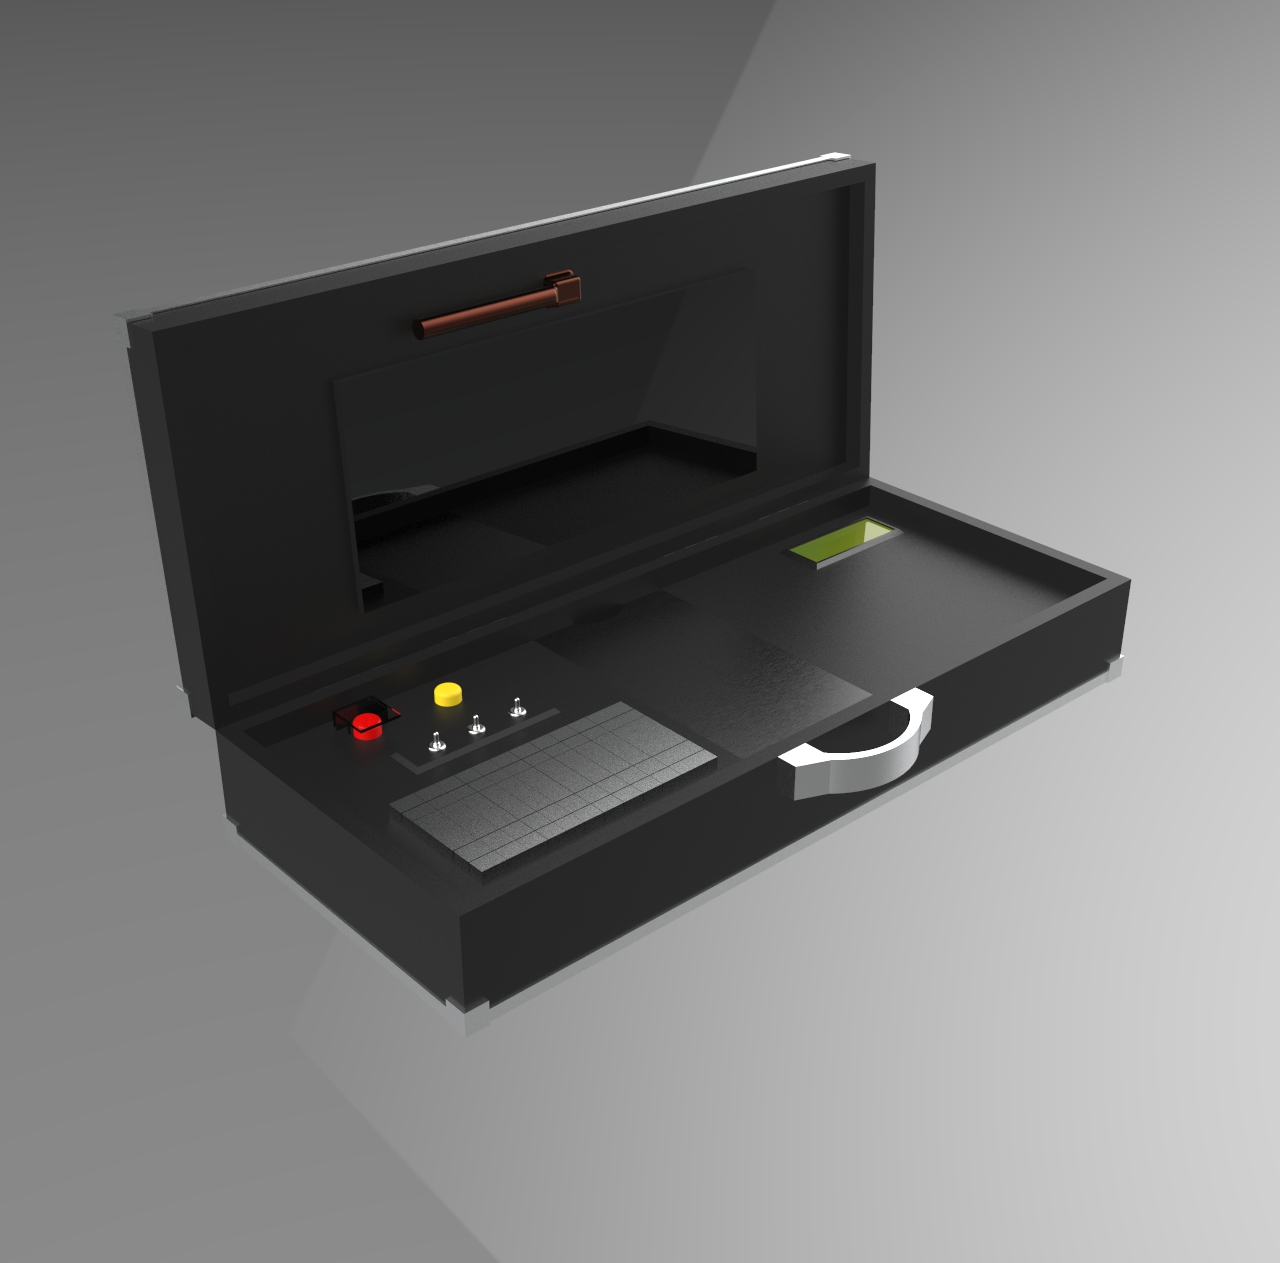
\includegraphics[width=0.9\textwidth]{figuras/maletaiso}
\caption{Maleta em visão isométrica }
\label{fig:maleta02}
\end{figure}

\subsubsection{Especificações de materiais}
\label{sub:Especificações de materiais}

\par Durante a seleção de materiais, é necessária uma sistematização que permita analisar a vasta possibilidade de combinação de materiais que podem constituir determinado produto a fim de extrair um candidato vencedor, que cumpre com maior eficiência possível os requisitos da aplicação \cite{walterconteudo}.

\par Antes de apresentar a lista em si, é necessário evidenciar as características desejáveis da caixa que será usada na \textit{ground station}. Durante a etapa de escolha do material a ser utilizado, nem sempre é possível contemplar satisfatoriamente todos os aspectos necessários para aquela determinada finalidade. Por isso, tais aspectos são dispostos em ordem de relevância para o projeto, para que a escolha do material seja feita com embasamento teórico dentro da necessidade real do protótipo. 

\par O fator mais relevante para a caixa da \textit{ground station} é o correto funcionamento no local de lançamento. A caixa deve estabelecer, por meio de ondas eletromagnéticas, comunicação mútua com o foguete e com o sistema de abastecimento de propelente durante todas as etapas de lançamento. Portanto, o material escolhido não deve gerar interferência nos sistemas de comunicação. 

\par A usabilidade e a ergonomia vem a seguir, responsáveis por garantir que o usuário consiga ler, de forma clara e precisa, todos os parâmetros relevantes para a missão e que o auxiliará na tomada de decisão. Assim, o material utilizado deve ser moldável para que embarque os componentes necessários e os disponha de maneira adequada, respeitando as suas diferentes geometrias.

\par O custo é o terceiro fator mais relevante, uma vez que a viabilidade de fabricação do protótipo está diretamente relacionada com seu valor final. Além do material ser acessível do ponto de vista financeiro, é desejável que ele permita agilidade em sua construção, dado que um material difícil de ser trabalhado pode gerar mais horas de trabalho, o que resulta no aumento do valor total da mão-de-obra e por consequência aumento do valor final do protótipo.

\par Como quarta prioridade, a caixa deve ser resistente de maneira que eventuais quedas ou impactos com outros objetos não venha a interferir o seu correto funcionamento. Materiais com boa resistência mecânica podem contemplar tal característica. 

\par Por fim, a portabilidade se faz necessária devida à utilização da caixa ocorrer lugares de acesso restrito. Logo, a caixa deve ser leve e compacta para facilitar o seu transporte.

\par Visto os aspectos desejáveis à caixa, é apresentado a seguir a sugestão de possíveis materiais a serem utilizados no protótipo.

\begin{itemize}
    \item \textbf{\textit{Medium Density Fiberboard} - MDF}
     \par O MDF é um material fabricado a partir da aglutinação de fibras de madeira com resina sintética – sendo as mais utilizadas à base de ureia formaldeído, tanino formaldeído e melamina ureia formaldeído –  posteriormente submetidas à prensagem em altas temperaturas  \cite{gomes}.  Sua composição permite que ondas eletromagnéticas possam fluir através dela.
     
    \par Sua superfície é plana e lisa, oferece alta usinabilidade para encaixar, entalhar, cortar, parafusar, perfurar e moldurar, além de reduzir o uso de tintas, vernizes e ótima aceitação de revestimentos \cite{CAMPOS}.
    
    \par O custo varia de acordo com a espessura da chapa. O valor do metro quadrado de uma chapa de 3 mm é R\$36,81. Já uma chapa de 6 mm custa R\$62,50 o metro quadrado.  Por possuir boa trabalhabilidade \cite{eleoterio2000propriedades}, o processo de construção pode apresentar satisfatória rapidez.  
    
    \par As características mecânicas específicas do material variam de acordo com o tipo de fibra e resina utilizadas. Em geral, são vantagens do MDF a alta relação entre resistência mecânica e massa específica, homogeneidade e ausência de defeitos como nós e desvios de grão \cite{eleoterio2000propriedades}. 
    
    \par De acordo com Silva e Gonçalves \cite{da2007avaliaccao}, os MDF são projetados para serem fabricados com densidades entre 0,5 e 0,8 $g/cm^3$.

    \item \textbf{Polímero Reforçado com Fibra de Vidro - PRFV}
    
    \par É um material composto por uma matriz de resina sintética termofixa, como a Resina Epóxi, reforçada com estreitos filamentos flexíveis de vidro, cujo principal constituinte é a sílica \cite{pierin2005estudo}. O PRFV não gera interferência na comunicação com os sistemas. 
    
    \par Possui razoável manuseabilidade, pode ser cortado, perfurado e moldado, porém caso a caixa seja composta por várias peças o encaixe entre elas pode dificultar o processo de montagem.    
    
    \par O processo de fabricação é lento pois é necessária a fabricação do PRFV em si, ou seja, não é vendido o PRFV pronto para uso e sim os filamentos de vidro e a resina. Além disso, o PRFV deve ser confeccionado em um molde que deve ser previamente fabricado com o formato da peça final. O custo de material suficiente para produzir um metro quadrado de PRFV é de R\$52,90.  
    
    \par De acordo com Lin et al (1996), conforme citado por Pierin \cite{pierin2005estudo}, os PRFV exibem alta resistência mecânica, porém problemas de deformabilidade e instabilidade, devido à sua baixa elasticidade e rigidez, são os maiores inconvenientes deste material. 
    
    \par De acordo com CALLISTER JR. \cite{callister2000ciencia}, a densidade do PRFV varia entre 1,5 $g/cm^3$ podendo chegar até próximo de 3 $g/cm^3$ dependendo dos materiais utilizados.
    
    \item \textbf{Polímero Reforçado com Fibra de Carbono - PRFC}
    \par Similar ao PRFV, o PRFC utiliza como reforço fibras compostas principalmente de carbono que resultam da pirólise de fibras plásticas, como a poliacrilonitrila (PAN). 
    
    \par O processo de fabricação do PRFC é análogo ao processo de fabricação do PRFV. O material para produzir um metro quadrado PRFC custa R\$421,43.
    
    \par Segundo Galli \cite{galli2016caracterizaccao} as fibras de carbono são normalmente empregadas em aplicações que requerem elevadas propriedades mecânicas (alta resistência mecânica e alto módulo de elasticidade) associadas a uma baixa densidade.
    
    \par Segundo o data sheet da HEXCEL a fibra de carbono apresenta uma densidade de 1,78 $g/cm^3$. \cite{datasheet_carbon}
    
    \item \textbf{Poli Ácido Lático - PLA}
    
    \par O PLA é um polímero termoplástico feito através da extração do milho, trigo ou cana de açúcar passando por várias etapas de produção. Sua composição permite o correto funcionamento dos sistemas de comunicação. 
    
	\par O PLA é um material comumente usado em prototipagem rápida onde uma impressora 3D deposita o material partindo de dados provenientes de sistemas de desenho assistido por computador (CAD). Sua alta fluidez e baixa contração durante o processo de extrusão permite a produção de peças com alta precisão dimensional e bom acabamento superficial.
	
	\par O filamento de PLA para impressão 3D tem valor médio de R\$140,00 o kg com a possibilidade e facilidade de poder encontrá-los em diversas cores. O valor de processamento do PLA para projetos com baixas unidades é muito elevado, tornando inviável seu processamento por injeção ou \textit{vacuum forming} e impressão 3D. 
	
	\par De acordo com Simões et al. \cite{simoes2009mechanical}, o PLA é um material rígido e resistente, difícil de deformar ou flexionar, possui alta dureza, que o torna com baixa resistência ao impacto. É um material indicado para produção de protótipos que não sejam submetidos às condições de altos esforços mecânicos, atritos ou altas temperaturas.
	
	\par De acordo com o experimento realizado por Santana et al. \cite{santana2018estudo} o PLA apresenta uma densidade de 1,24 $g/cm^3$.

    \item \textbf{Acrilonitrila Butadieno Estireno - ABS}
    
    \par Para  Vossen  \cite{vossen2009nanocompositos},  o  ABS é  um  termoplástico  que  consiste em uma  fase  de  borracha  (butadieno)  dispersa  em  uma  matriz de  SAN  (copolímero  de  acrilonitrila  Estireno),  também denominado terpolímero.
    
	\par A acrilonitrila confere estabilidade ao calor e resistência química e à flexão; o butadieno é responsável pela resistência ao impacto e tenacidade; já o estireno por sua vez é responsável pelo brilho, rigidez e fácil processamento. Devido à suas propriedade e baixo custo o ABS se tornou um material bastante utilizado por várias indústrias. O ABS pode ser Processado por injeção, extrusão e sopro.
	
	\par O valor do ABS depende da forma em que você o deseja, o kg do ABS granulado custa em média R\$ 16,80 já o kg do filamento (399 m) de ABS para impressão varia de R\$50,00 a R\$100,00. O valor de processamento do ABS para projetos com baixas unidades é muito elevado, tornando inviável seu processamento por injeção ou \textit{vacuum forming} e impressão 3D.
	
	\par Assim as propriedades do ABS dependem do teor de cada componente, mas em geral o ABS apresenta boa resistência térmica e ao impacto, alta estabilidade dimensional, alta rigidez, alta dureza, baixa absorção de umidade, etc. \cite{junior2014aspectos}
	\par O ABS apresenta uma densidade de 1,04 $g/cm^3$.

\end{itemize}

\paragraph{Quadro comparativo na escolha de materiais:}

\par Na confecção do quadro comparativo, foi atribuído um grau de satisfação de cada material de acordo com o requisito desejado. Este grau varia em três níveis: bom, razoável e ruim. Coube aos autores do presente trabalho definir o grau de satisfação de acordo com suas interpretações das informações dispostas anteriormente. O resultado é mostrado na tabela \ref{tab:materiais}.

\begin{table}[!h]
\centering
\begin{tabular}{|l|l|l|l|l|l|}
\hline
 & MDF & PRFV     & PRFC     & PLA      & ABS      \\ \hline
\begin{tabular}[c]{@{}l@{}}Comunicação com \\ os subsistemas\end{tabular} & Bom & Bom      & Bom      & Bom      & Bom      \\ \hline
\begin{tabular}[c]{@{}l@{}}Usabilidade e \\ ergonomia\end{tabular}        & Bom & Razoável & Razoável & Bom      & Bom      \\ \hline
Custo                                                                     & Bom & Bom      & Ruim     & Razoável & Razoável \\ \hline
\begin{tabular}[c]{@{}l@{}}Propriedades \\ mecânicas\end{tabular}         & Bom & Razoável & Bom      & Razoável & Razoável \\ \hline
Densidade                                                                 & Bom & Razoável & Bom      & Bom      & Bom      \\ \hline
\end{tabular}
\caption{Quadro comparativo de escolha de materiais}
\label{tab:materiais}
\end{table}

\par De acordo com o resultado da tabela \ref{tab:materiais}, o material propício para a confecção do protótipo é o \textbf{MDF}.

\par Walter sinaliza que a dinâmica de Seleção de Materiais e Processos de Fabricação devem ser flexíveis a ponto de permitir sua utilização em etapas desde o Design Conceitual ao Projeto para Manufatura \cite{walterconteudo}. 

\par Se tratando de um projeto de engenharia, é possível que se escolha mais de um material, já que suas partes possuem funções diferentes. Por exemplo, a carcaça da caixa pode ser feita em PLA ou ABS, o que permite um acabamento melhorado e uma proteção em caso de eventual contato com líquidos. Já os componentes estruturais podem ser feitos em MDF, o que acarretaria na diminuição dos custos de produção, diminuição do peso e aumento das propriedades mecânicas se comparado aos polímeros.

\subsection{Abastecimento}

\par No referente trabalho o abastecimento é todo o conjunto que engloba o sistema de alimentação e os processos necessários para que o propelente líquido seja transferido para o foguete de forma remota, segura e no momento indicado pelo usuário.

\subsubsection{Elementos do sistema de alimentação}

\par A seguir é apresentado um fluxograma do sistema de alimentação, figura \ref{fig:sistema de alimentacao}, onde logo depois é caracterizado e especificado cada componente pré estabelecido pelo cliente, em anexo \ref{ane:Elementos do sistema de alimentação} é apresentada as imagens de cada um dos elementos descritos aqui.

\begin{figure}[H]
\centering
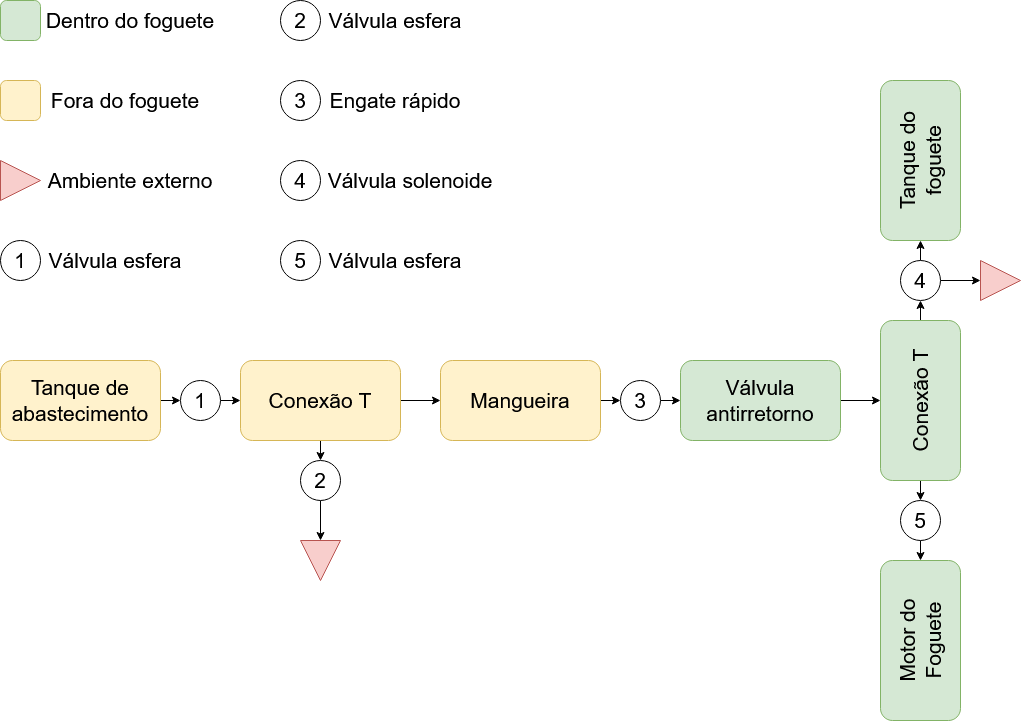
\includegraphics[width=0.9\textwidth]{figuras/diagramaAlimentacao}
\caption{Fluxograma do sistema de alimentação}
\label{fig:sistema de alimentacao}
\end{figure}

\begin{enumerate}
\begin{enumerate}[a]
    \item \textbf{Tanque de abastecimento}: É um cilindro comercial fornecido pela empresa distribuidora de óxido nitroso. A válvula esfera, item 1 da figura \ref{fig:sistema de alimentacao}, deverá ser conectada no bocal de saída desse cilindro, com uso de adaptador caso necessário.
    \item \textbf{Válvula esfera macho-fêmea 1/2 polegada NPT}: É uma válvula de abertura de 90º. Seu manípulo deverá ser retirado e a haste ligada à esfera de abertura/fechamento será conectada ao mecanismo eletromecânico de abertura. 
    \item \textbf{Conector em T macho-fêmea-macho 1/2 polegada NPT}: São adaptadores em pontos de bifurcação do sistema hidráulico.
    \item \textbf{Tubo flexível 1/2 polegada de aço inox com tramas de aço}: É necessário por não reagir com o óxido nitroso, como ocorre com a borracha, comum nas mangueiras convencionais.
    \item \textbf{Engate rápido 3/4 polegada NPT}: É uma conexão composta por duas peças (macho e fêmea) e um anel de segurança. Somente movendo o anel é que as duas peças podem ser desconectadas.
    \item \textbf{Válvula anti-retorno macho-fêmea 3/4 polegada NPT}: É uma válvula de sentido único, ligada ao engate rápido da mangueira e o conector T que liga o tanque ao motor dentro do foguete. Evita que o óxido nitroso volte no sentido do tanque de abastecimento.
    
\end{enumerate}
\end{enumerate}

\subsubsection{Funcionamento do sistema de abastecimento}
\par Com base no projeto desenvolvido pelo cliente \cite{capitalrocketteam2020}, o funcionamento do sistema de abastecimento ocorre em etapas, cada uma delas correspondendo a estados das válvulas se estão abertas ou fechadas, figura \ref{fig:sistema de alimentacao}, conforme a ação desejada. 

\begin{enumerate}
    \item \textbf{Etapa 1 - Estado inicial}: todas as válvulas estarão fechadas, ou seja, o sistema estará em repouso, de modo a evitar qualquer vazamento antes do início do processo de abastecimento; 
    
    \item \textbf{Etapa 2 - Resfriamento do tanque do foguete}: abertura das válvulas 1 e 4, de modo a realizar a passagem de um fluxo inicial do fluido oxidante, com a finalidade de resfriar o tanque do foguete e otimizar seu abastecimento. O tempo de resfriamento fica a critério do usuário, e a etapa é encerrada com o fechamento das duas válvulas;
    
    \item \textbf{Etapa 3 - Abastecimento do tanque}: abertura da válvula 1, com posterior abertura e fechamento intermitente da válvula 4 para alívio da pressão interna do tanque do foguete durante seu abastecimento. O fluido oxidante é transportado, devido a fenômenos termodinâmicos, em estado de mistura (líquido e gás), e no tanque do foguete a sua fase gasosa deverá ser expulsa pela válvula 4, até o nível definido pelo usuário, este é controlado pela célula de carga que mede a variação de peso do foguete. Com base nos dados fornecidos pela célula de carga, o usuário avaliará se o tanque se encontra cheio, encerrando a etapa com o fechamento da válvula 1 e, caso aberta, da válvula 4; 
    \item \textbf{Etapa 4 - Alívio de pressão da mangueira}: abertura da válvula 2 para expurgo do fluido oxidante que se encontra no interior da mangueira, de modo a equalizar sua pressão interna com a pressão ambiente, de modo a ser possível realizar seu desacoplamento do foguete. A existência de uma válvula anti-retorno na linha de abastecimento impede que o fluido contido no tanque do foguete seja também expurgado nessa fase; 
    \item \textbf{Etapa 5 - Desacoplamento da mangueira}: acionamento do engate rápido, por meio de um atuador linear, de modo a desacoplar e afastar a mangueira do foguete. Essa etapa encerra o processo de abastecimento, e o foguete está preparado para o lançamento; 
    \item \textbf{Etapa 6 - Ignição do foguete}: após o acionamento do ignitor junto ao combustível no motor do foguete, por meio do comando da estação de controle, é feita a abertura da válvula 5, que injetará o fluido oxidante do tanque do foguete na câmara de combustão no interior do motor. Assim o encontro desse fluido com o combustível e o calor gerado pelo ignitor iniciará a combustão principal, e o foguete iniciará sua decolagem.
\end{enumerate}

\subsubsection{Características do abastecimento}

\par Como mencionado, durante o transporte do fluido oxidante do tanque de abastecimento para o tanque do foguete, fenômenos termodinâmicos ocorrem, como a queda de temperatura provocada pela passagem do fluido conforme ele vai reduzindo a pressão à qual estava submetido no cilindro comercial (por volta de 50 bar). Em alguns casos, esse fenômeno é desejável, como para o resfriamento do tanque do foguete, em outros, ele pode apresentar um problema, como o congelamento de válvulas e atuadores que não estejam nas especificações adequadas. Do mesmo modo, a atuação das válvulas ocorrerá em situações em que o fluido estará a grande pressão, o que impede o manuseio delas manualmente, seja por necessidade, seja por questões de segurança. Ademais, não é recomendado o uso de mangueiras muito longas para o abastecimento, devido à perda do fluido durante seu transporte.

\par A solução proposta é o acoplamento de dois atuadores rotativos nas válvulas 1 e 2, bem como de um atuador linear no engate rápido, 3, os quais receberão um comando remoto de abertura e fechamento a partir da estação de controle. Para tanto, será necessário tanto o dimensionamento das opções comerciais para atuadores, desde o torque gerado por cada um dos modelos até sua natureza – se eletrônico ou pneumático, quanto o desenvolvimento de uma estrutura de suporte e adaptação entre esses atuadores e as válvulas e conexões do sistema de alimentação, a qual também deverá observar as características (variação de temperatura e pressão) do processo der abastecimento. 

\subsubsection{Atuadores elétricos ou pneumáticos}

\par \textbf{Usabilidade}: Atuadores elétricos, figura \ref{fig:atuador eletrico}, são peças únicas que necessitam de uma fonte de energia para funcionar, enquanto atuadores pneumáticos, figura \ref{fig:atuador pneumatico}, necessitam de um fluido trabalho (ar comprimido, gás inerte, etc) que gera a pressão necessária para atuar sobre a válvula. Isso requer um sistema hidráulico acessório ao sistema de alimentação principal, com um conjunto próprio de mangueiras e tanque de abastecimento. Porém, no caso dos atuadores elétricos, as soluções comerciais normalmente voltadas para abertura de válvulas exigem uma fonte de tensão de 24V, o que está além do dimensionamento energético feito para o presente projeto;

\begin{figure}[h]
\centering
\subfigure[ref1][Atuador 24V] {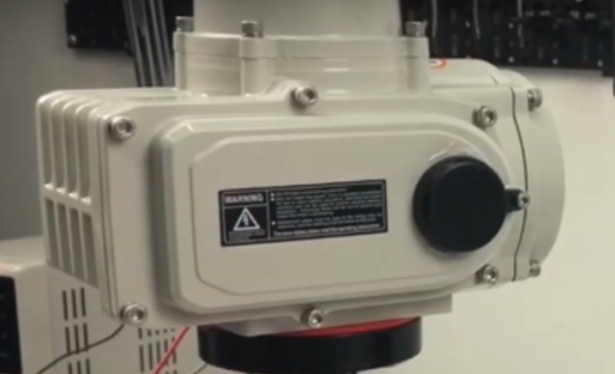
\includegraphics[width=7cm]{figuras/atuadorEletrico24V.png}}
\qquad
\subfigure[ref2][Atuador 12V] {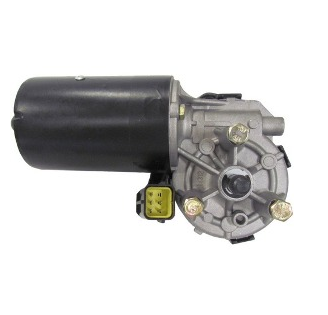
\includegraphics[width=6cm]{figuras/atuadorEletrico12V.png}}
\caption{Atuadores elétricos}
\label{fig:atuador eletrico}
\end{figure}

\par \textbf{Atuação}: Um atuador elétrico é mais demorado para exercer a rotação sobre a válvula, de 10 a 20 segundos a depender do modelo. Enquanto que o atuador pneumático, por sua vez, tem atuação praticamente imediata, 1 segundo ou menos, a partir do comando de abertura ou fechamento;

\par \textbf{Acessibilidade}: Atuadores pneumáticos são mais comuns de serem encontrados no Brasil, enquanto que os elétricos são mais comumente encontrados em casas de importação ou comércio eletrônico de importação. É importante ressaltar ainda que esses atuadores são mais robustos dos que os servomotores normalmente encontrados em comércios de componentes eletrônicos, os quais não necessitam gerar torques muito grandes;

\par \textbf{Segurança}: Atuadores pneumáticos são mais recomendados em locais potencialmente explosivos, por não apresentar riscos de soltar faíscas que provoquem um acidente. Ao mesmo tempo, em caso de queda de energia (ou de pressão no caso do pneumático), ambos os atuadores permanecem no mesmo estado que se encontram, a menos que se opte por modelos que utilizem-se de bateria ou sistema de molas, para cada caso respectivamente. Já que estes permitem que eles sejam configuráveis para voltar ao estado aberto ou fechado em caso de falha;

\par \textbf{Torque e preço}: A capacidade de torque varia de acordo com o modelo e, no caso do atuador pneumático, com a pressão do ar comprimido que pode ir de 2 a mais de 6000 $N.m$. O preço de um atuador pneumático, nesse contexto, pode variar de 250 a 2000 reais, podendo chegar a mais de 14 mil reais, em casos específicos de aplicação industrial. Alguns atuadores elétricos podem ser encontrados por valores entre 60 e 240 dólares (não contando frete ou taxas de importação). Esses valores podem variar conforme o fornecedor ou casa de importação, os quais normalmente disponibilizam o valor dessas peças somente mediante solicitação de orçamento.

\begin{figure}[!h]
\centering
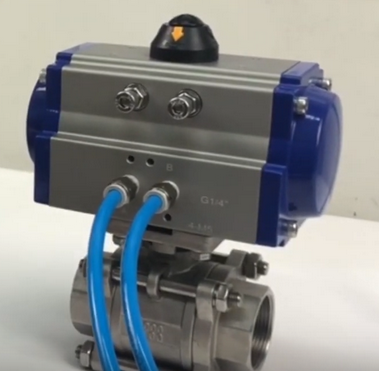
\includegraphics[width=0.5\textwidth]{figuras/atuadorPneumatico.png}
\caption{Atuador Pneumático}
\label{fig:atuador pneumatico}
\end{figure}

\par Como regra geral, é de se esperar que o atuador elétrico seja mais caro que o atuador pneumático, para a mesma aplicação, ressalvando-se a necessidade de um sistema hidráulico adicional para o caso deste último.